Parámetros del test: 
Cantidad de iteraciones por filtro-version 20.
empieza con un corte de 16x2144 y va restando al alto 16 y sumando al ancho la misma cantidad hasta llegar a 2144x16. tiene offsetX = 0 y offsetY = 500.

\begin{figure}[h]
  \begin{center}
	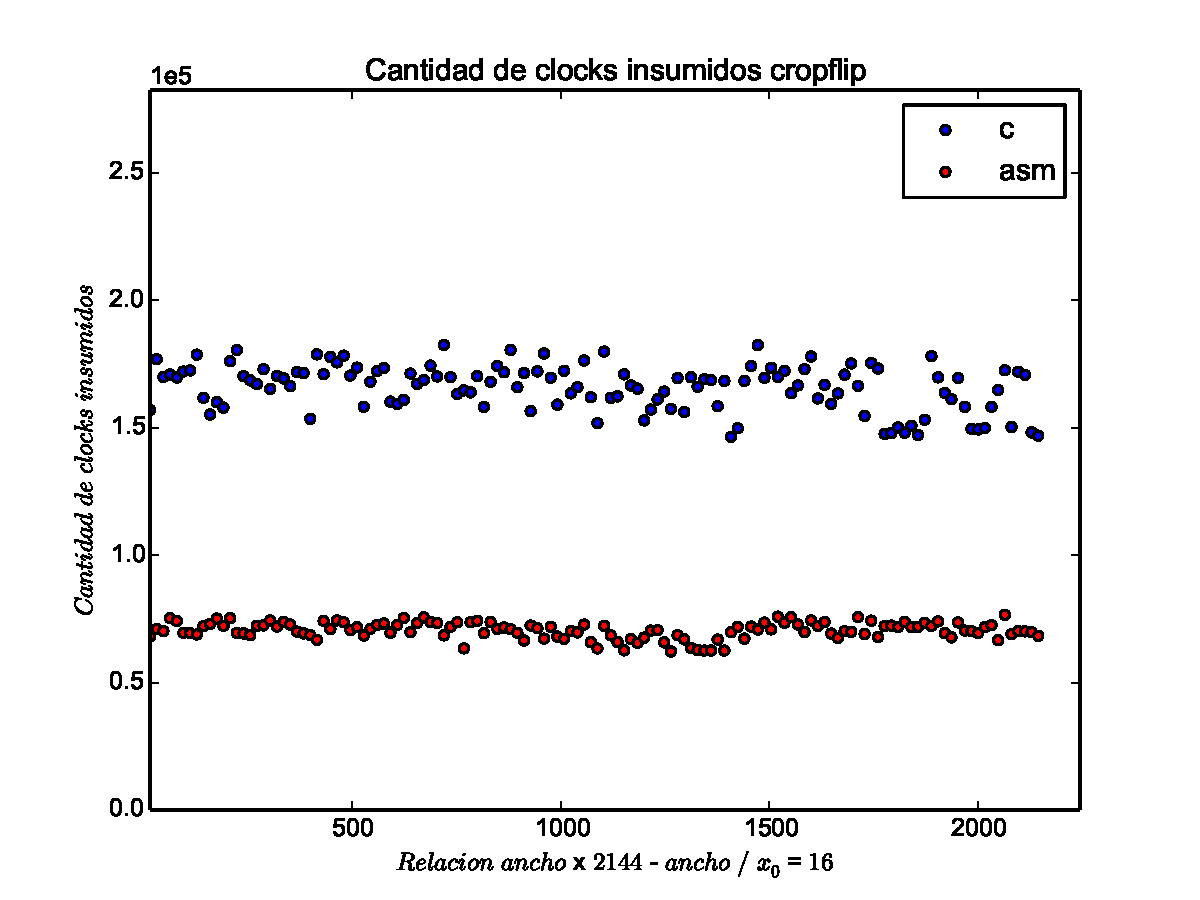
\includegraphics[scale=0.5]{cachecropflip.pdf}
	%\caption{La última de Star Wars}
  \end{center}
\end{figure}


Observamos que el tiempo insumido en las diferentes corridas se mantiene comparativamente constante. Por lo cual, concluimos que la cache no parece ser un factor tan relevante en este caso como suponiamos. 
\newpage